\documentclass[a3paper,extrafontsizes,20pt, ngerman]{memoir}

\usepackage{pgfplots}
\usepackage{caption}

\renewcommand{\familydefault}{\sfdefault}
\usepackage[landscape, left=1cm, right=1cm, top=1cm, bottom=1cm]{geometry}

\begin{document}

\begin{figure}
    \centering
    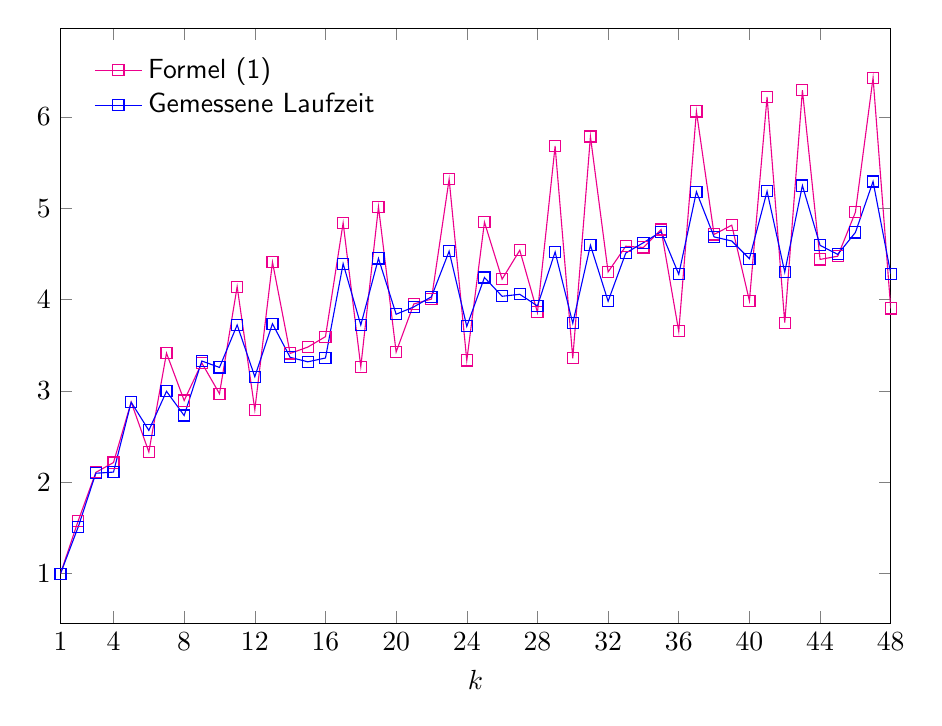
\begin{tikzpicture}
        \begin{axis}[
                xlabel = {$k$},
                xmin = 1,
                xmax = 48,
                xtick = {1, 4, 8, 12, 16, 20, 24, 28, 32, 36, 40, 44, 48},
                width = \textwidth,
                height = 260pt,
                legend pos = north west,
                legend style = {draw = none, scale = 1.4,},
                legend cell align = left,
            ]

            \addplot[color=magenta,mark=square]
            coordinates{
                    (1, 1.0)
                    (2, 1.5773502691896257)
                    (3, 2.1086517918741277)
                    (4, 2.21648605664914)
                    (5, 2.8790043489023804)
                    (6, 2.332272327437964)
                    (7, 3.414299970503978)
                    (8, 2.89543195056782)
                    (9, 3.3067332978837425)
                    (10, 2.970093877947532)
                    (11, 4.142494904167608)
                    (12, 2.7949482208102387)
                    (13, 4.411181889332409)
                    (14, 3.4111279805567123)
                    (15, 3.481018974295858)
                    (16, 3.594729442047154)
                    (17, 4.840295239186588)
                    (18, 3.2665648302249286)
                    (19, 5.017128905823505)
                    (20, 3.426648342312123)
                    (21, 3.952865384732847)
                    (22, 4.006284568144385)
                    (23, 5.319207262349245)
                    (24, 3.3342189545431045)
                    (25, 4.848341222073144)
                    (26, 4.224515025049569)
                    (27, 4.541184581320172)
                    (28, 3.8606214340939586)
                    (29, 5.682737117278753)
                    (30, 3.3580839014528188)
                    (31, 5.786717613861166)
                    (32, 4.303622115889641)
                    (33, 4.585058767874234)
                    (34, 4.57165798930078)
                    (35, 4.768544753994481)
                    (36, 3.65286546982577)
                    (37, 6.061272505622063)
                    (38, 4.714254318317245)
                    (39, 4.815669489895146)
                    (40, 3.9872807230736402)
                    (41, 6.219718898826906)
                    (42, 3.7480426730792065)
                    (43, 6.293026650584624)
                    (44, 4.440755450349039)
                    (45, 4.475806923989725)
                    (46, 4.957283888509379)
                    (47, 6.429590774020685)
                    (48, 3.903718627468377)
                };

            \addplot[color=blue,mark=square]
            coordinates {
                    (1, 1.0)
                    (2, 1.509948118652118)
                    (3, 2.0993697474766457)
                    (4, 2.1116345085043)
                    (5, 2.877418891483742)
                    (6, 2.5685036940000137)
                    (7, 2.996430188276255)
                    (8, 2.7314845124186458)
                    (9, 3.328296749381993)
                    (10, 3.2577944117129998)
                    (11, 3.7230055520415988)
                    (12, 3.1561945991451923)
                    (13, 3.736074156058803)
                    (14, 3.3685945128552692)
                    (15, 3.319276959371872)
                    (16, 3.3613292919244078)
                    (17, 4.394228617904989)
                    (18, 3.722443809049611)
                    (19, 4.451548228110135)
                    (20, 3.84047914786071)
                    (21, 3.920376539331896)
                    (22, 4.032026952636839)
                    (23, 4.529968590050905)
                    (24, 3.707477302822801)
                    (25, 4.242901333931946)
                    (26, 4.037016391081217)
                    (27, 4.058783598622834)
                    (28, 3.9310913363101916)
                    (29, 4.522555243332595)
                    (30, 3.7415823259420846)
                    (31, 4.59640961602802)
                    (32, 3.982932254189798)
                    (33, 4.510560919218005)
                    (34, 4.624088329155094)
                    (35, 4.744870700917283)
                    (36, 4.277919837533675)
                    (37, 5.181576815360558)
                    (38, 4.687283294435714)
                    (39, 4.642788634977157)
                    (40, 4.449130421846238)
                    (41, 5.186842863188695)
                    (42, 4.302098653348379)
                    (43, 5.24978349062113)
                    (44, 4.594828700423131)
                    (45, 4.4958880668775825)
                    (46, 4.73608695893801)
                    (47, 5.293961293662393)
                    (48, 4.28487474982348)};

            \legend{Formel (1), Gemessene Laufzeit}
        \end{axis}
    \end{tikzpicture}
    \captionsetup{labelformat=empty}
    \caption{Abbildung 1: Die gemessene Laufzeit und Werte von Formel (1) für $M = 1$ und $1 \le k \le 48$. Alle Werte sind relativ bzgl. $k = 1$.}
\end{figure}
\end{document}